\section{Introduction}

\subsection{Examples of Machine Learning}
\begin{itemize}
	\item The things listed here are just here to provide a sense of what machine learning can
		be useful for. It's not a complete list (obviously), and we will spend time
		throughout the semester learning about some of these things. 
		\begin{enumerate}[label=\roman*.]
			\item Recognizing digits in images -- this is something that people have spent a
				lot of time trying to fine tune historically. Nowadays we have it figured
				out, but it took a surprising amount of time to get this right. 
			\item Identifying a tumor in an x-ray
			\item Classifying email as spam
			\item Diagnosing a disease from symptoms
			\item Predicting the price of a stock 6 months into the future. 
			\item Predicting the 3D structure of all atoms in a protein from it's amino acid
				structure. 
		\end{enumerate}
		There are also many types of learning problems in machine learning: 
		\begin{itemize}
			\item \textit{Classification Problems}: where the output is a label from a finite
				set. 
			\item \textit{Regression Problems}: the output is real-valued 
			\item \textit{Ranking Problems}: the output only ranks examples relative
				to one another.
			\item \textit{Unsupervised Problems}: models like Chat-GPT, are used for
				generative problems. 
		\end{itemize}
\end{itemize}
\subsection{MNIST}
\begin{itemize}
	\item This is a training set of 60,000+ examples, which was a very popular dataset to grade
		ML model performance. Each digit is a 28x28 pixel of a grey level image, and the goal
		is to have a machine identify what each number is. 
	\item In essence, you can think of each
		input as a matrix with a real valued number in it.
	\item Nowadays, we've managed to get
		the error rate down to somewhere around 0.5\%. 

\end{itemize}

\subsection{Machine Learning Approach}
\begin{itemize}
	\item Essentially, the thing we are training is what's called "feature vectors", which
		train a classifier, done in what's called "training time". 
	\item At training time, the classifier then takes in new data on an untrained 
		dataset,
		and classifies them (test time). This test dataset is usually a dataset 
		in which we
		know the correct answer, which helps us evaluate how well the model behaves. 
	\item Finally, we deploy this model for its intended use. Shockingly, 
		this is the one that's easiest to forget. 
	\item In the case of training images, we turn the 2x2 matrix of image intensities 
		into a vector instead, and classify the vector 
		(this is the same process as before, no data
		is being destroyed here). 

	\item Suppose we're training a model, and our dataset looks like:

		\begin{center}
			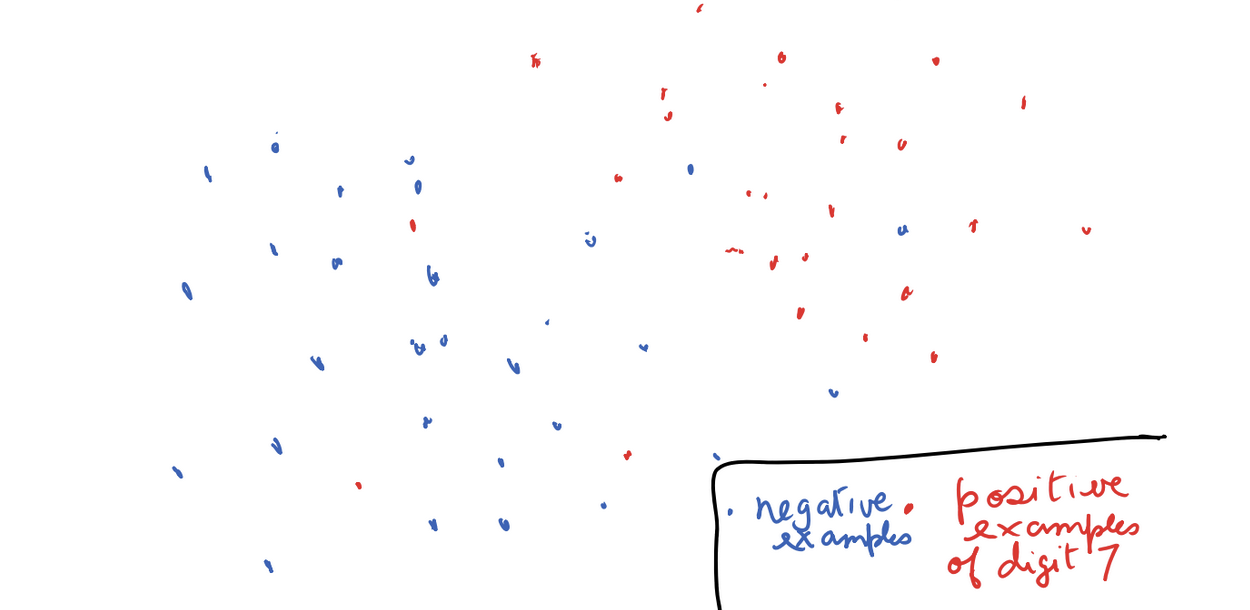
\includegraphics[scale=0.4]{lec-1a.png}
		\end{center}

		Let's say that the red dots are "positive" examples of the digit 7, and the 
		blue dots represent "negative examples" (not a 7). 
		Now, if we get a new point, how do
		we classify it?
	\item One way we can do this is via \textit{nearest neighbors}, which basically
		finds the point closest to the new data point, and classifies it as such. The
		idea here is that the similarity between the new point is highest with its
		nearest neighbor, so the probability it classifies in the same way is also
		the highest.
	\item There is also the idea of a linear classifier, where we draw a line \(
		\tilde w \cdot \tilde x + b = 0 \), which gives us a way to classify new
		point based on where they fall relative to that boundary.   
	\item Sometimes, linear classifiers aren't good enough. If our distribution is
		less skewed, then sometimes a single line isn't very effective. Sometimes, we
		can even have multiple boundaries, making the entire thing highly nonlinear.   
\end{itemize}
\subsubsection{Small aside on training error} 
\begin{itemize}
	\item Is it good to have zero training error? Yes, but only if you have a LOT of
		data. Companies like Google, Microsoft. etc. work with incredibly large
		datasets, in which case for them zero training error is a target, but if
		we're working with a smaller dataset (which will be the case at most
		companies except the largest ones), having some training error may actually
		be a good thing. 
	\item Having zero training error means that the model has basically memorized the
		training data, so there's absolutely no way that this model can be good
		elsewhere. \question{why is this?}    
\end{itemize}

\subsection{How to make nonlinear decision boundaries?}
\begin{itemize}
	\item Nearest neighbors gives us a nonlinear decision boundary, and it gets
		pretty good once we start considering multiple neighbors. 
	\item One other way we can do this is to use Neural networks to basically make
		better feature vectors directly from the initial ones. At the end, it
		generates a linear decision boundary. This is called the "latent
		representation". Then, we can build a classifier on top
		of this decision boundary. In essence, this is what a linear classifier does. 
	\item Suppose all the positive examples lie inside a disk. Then, there's no
		possible way for a linear classifier to work well on the initial data, but
		the hope is that we can use machine learning to generate another feature
		space where a linear classifier \textit{would} work.    

		For the disk example, we could take a boundary \( x_1^2 + x_2^2 = c \), then
		the classification is linear with respect to \( x_1^2 \) and \( x_2^2 \)!
		Therefore, we can perform a linear classification here. In our case, our
		features could be:
		\[
			\begin{bmatrix} x_1 \\ x_2 \\ x_1^2 \\ x_1x_2 \\ x_2^2 \end{bmatrix}
		\]
		Note that this doesn't change our data at all, it just modifies it in a way
		so that we can perform linear regression on it. Here, we would try to find
		a linear classifier in this 5-dimensional space.       
\end{itemize}

\subsection{Neural Networks}
\begin{itemize}
	\item All they are is just composing simple logistic regression functions over
		and over again.  
	\item For a single layer, single output neural network, it would take each input,
		and have its own weight \( w_i \) associated with them. Then, we can output
		something along the lines of:
		\[
			v_2 = \sum_k w_{k}x_k 
		\]
		In other words, we can think of this as an inner product between our input
		and the weight vector.   
	\item Then, what we will do is to introduce some nonlinearity into the equation,
		so that we can get something meaningful out of the neural network. If we just
		keep repeating this with linear functions, then we're obviously going to get
		something linear as output, which doesn't help us.
	\item In linear regression, one function we may choose to use is the sigmoid
		function, written as:
		\[
			g(z) = \frac{1}{1 + e^{-z}}
		\]
		and we output \( v_2 = g(\sum_k w_kx_k) \). Now that we pass the dot product
		through a nonlinear function, then we now get something more meaningful.
	\item Sometimes, these functions \( g(z) \) are called \textit{activation
		functions}. We can put these in between layers as well. 
	\item Now we can push this to multiple layers, where we have a layer in between
		our input and output:
		\begin{center}
			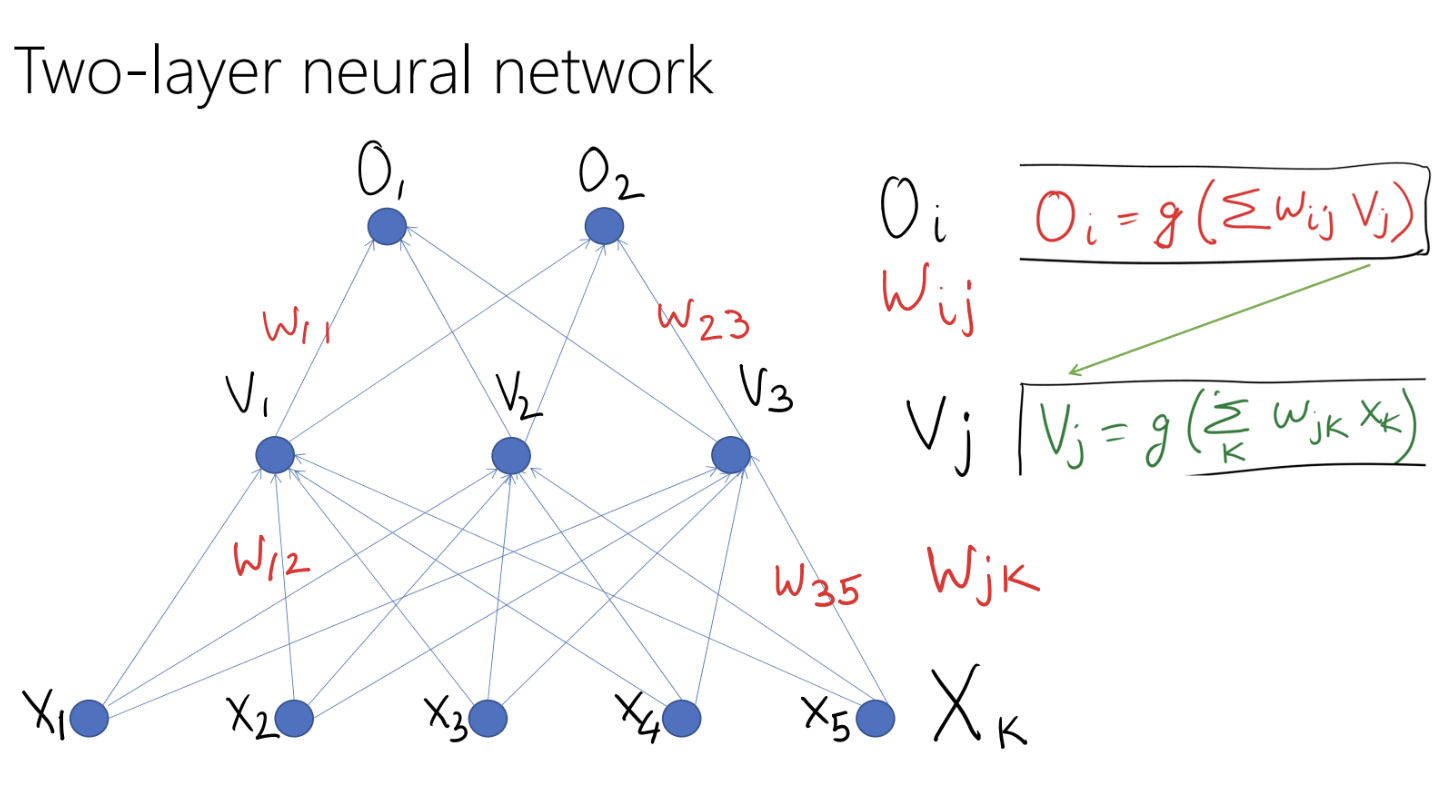
\includegraphics[scale=0.4]{lec-1b.png}
		\end{center}
		Notice how the \( v_i \) gets pushed through our activation function, and so
		does our \( o_i \). Because of the way information is passed from layer to
		layer, this is sometimes called a \textit{feed-forward} neural network.
		If we put it all together, we get:
		\[
			o_i = g\left( \sum_j w_{ij} g\left( \sum_k w_{jk} x_k \right) \right)
		\]
\end{itemize}
\subsection{Training a Neural Network}
\begin{itemize}
	\item At the end of the day, the goal is to find a \( w \), such that \( o_i \)
		is as close as possible to the true label (or true output). If this
		probability is low, then we have a bad setting of the parameters.  
	\item To do this, we can define a loss function \( \mathcal{L}(w) \), and compute
		\( \nabla_w \mathcal{L} \). Then, we update \( w \) by:
		\[
			w_{\text{new}} = w_\text{old} - \eta \nabla_w\mathcal{L}
		\]
		The value of \( \eta \) is called a \textbf{hyperparameter} which we set prior
		to running the training procedure. This process is known as 
		\textbf{gradient descent}. More complicated
		optimization procedures do exist, but they're basically never used in
		practical machine learning.  
	\item Now, the question is, what kind of loss function \( \mathcal{L} \) should
		we use? 
	\item A good choice for a loss function is the likelihood (also known as
		cross-entropy):
		\[
			\mathcal{L} = -\sum_\text{input data}(y_i \ln o_i + (1 - y_i) \ln( 1 -
			o_i) 
		\]
		It turns out, using this as our loss function actually reduces the problem
		directly to logistic regression!  
\end{itemize}
